\documentclass[a4paper,12pt]{article}
\usepackage[utf8]{inputenc}
\usepackage[T1]{fontenc}
\usepackage{graphicx}
\usepackage{listings}
\usepackage{caption}
\usepackage{tocloft}
\usepackage[margin=1in]{geometry}
\usepackage[polish]{babel}
\usepackage{fancyvrb}

\lstset{
	language=C++,
	basicstyle=\ttfamily,
	numbers=left,
	numberstyle=\tiny,
	stepnumber=1,
	numbersep=5pt,
	tabsize=4,
	captionpos=b,
	breaklines=true,
	breakatwhitespace=false,
	frame=single,
	showstringspaces=false,
}
\renewcommand{\cftsecleader}{\cftdotfill{\cftdotsep}}
\renewcommand{\listfigurename}{Spis rysunków}
\renewcommand{\listtablename}{Spis tabel}

\begin{document}
	\begin{titlepage}
		\centering
		\vspace*{1cm}
		\Huge \textbf{Dokumentacja techniczna do obsługi aplikacji bankowej}\\
		
		\vspace{1.5cm}
		\vspace{10cm}
		\Large Autorzy: \\Magdalena Denicka\\ Andrii Zapukhlyi \\
		\vspace{2cm}
\today
		\vfill
	\end{titlepage}
	
	\tableofcontents
	\newpage
	

	\section{Wprowadzenie}
	
	Witamy w dokumentacji technicznej aplikacji do obsługi bankowości, stworzonej z myślą o zapewnieniu pracownikom intuicyjnego i prostego operowania. Dokument ten stanowi źródło informacji dla osób zainteresowanych zrozumieniem architektury i funkcji aplikacji.
	
	Głównym celem aplikacji jest umożliwienie pracownikom banku łatwych, efektywnych i bezpiecznych operacji niezbędnych do bezproblemowego działania banku.
	
	Dokumentacja została podzielona na oddzielne rozdziały, aby ułatwić zrozumienie różnych elementów aplikacji. 
	
	\section{Funkcje aplikacji i interfejs}
	Rozdział dotyczy najważniejszych funkcjonalności aplikacji, niezbędnych do poprawnego działania banku. Poniżej lista funkcji aplikacji:
	\begin{itemize}
		\item Tworzenie i usuwanie konta bankowego
		\item Operacje na środkach – depozyty oraz wycofywanie
		\item Wgląd na saldo konkretnego konta
		\item Zlecanie przelewów między kontami bankowymi
		\item Wgląd na listę wszystkich użytkowników bankowości
		\item Modyfikacja danych konta
		\item Zapis kont do zewnętrznego pliku
	\end{itemize}
Interfejs został zaprojektowany tak, aby był zrozumiały dla każdej osoby używającej aplikacji. 
Oparty jest o osiem funkcjonalnych przycisków przedstawionych na rysunku \ref{wyglad}.

	\begin{figure}[h]
		\centering
		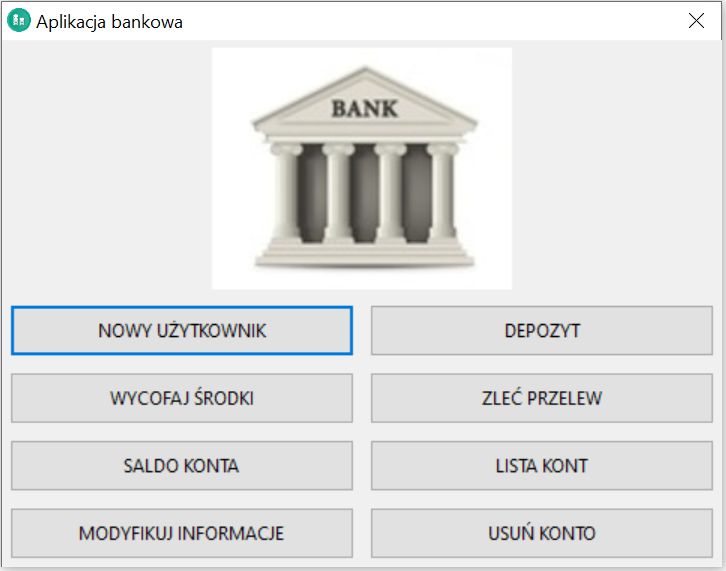
\includegraphics[width=0.6\textwidth]{wyglad.png}
		\caption{Wygląd aplikacji bankowej}
		\label{wyglad}
	\end{figure}


	\newpage
	\section{Dodawanie konta bankowego}
	Aby dodać nowe konto bankowe w aplikacji, należy:
	\begin{enumerate}
		\item Otworzyć aplikację bankowości
		\item Kliknąć przycisk ‘\textbf{NOWY UŻYTKOWNIK}’
		\item W polu „Nr konta” wpisać numer konta dodawanego użytkownika
		\item W polu „Imię” wpisać pełne imię użytkownika
		\item W polu „Nazwisko” wpisać pełne nazwisko użytkownika
		\item W polu „Saldo konta” wpisać początkowy stan konta użytkownika w formie liczbowej
		\item Kliknąć przycisk ‘\textbf{DODAJ UŻYTKOWNIKA}’ po wprowadzeniu i weryfikacji danych
	\end{enumerate}
		\begin{figure}[h]
		\centering
		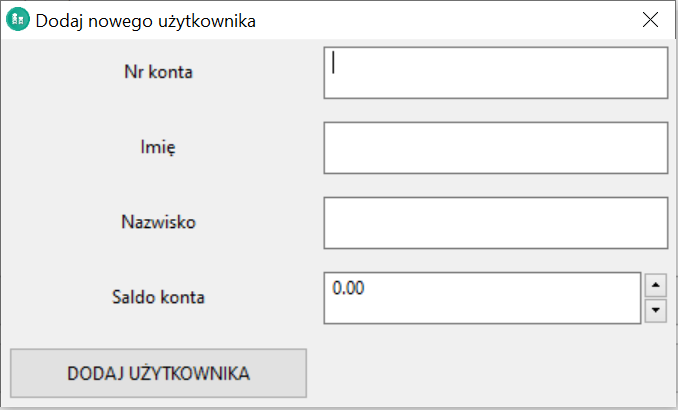
\includegraphics[width=0.8\textwidth]{new_user.png}
		\caption{Dodawanie nowego użytkownika}
		\label{new_user}
	\end{figure}
\newpage
\subsection{Kod źródłowy}
Sprawdzamy, czy podany numer konta istnieje w pliku db.txt. Jeśli plik jest otwarty, funkcja przechodzi do pętli while. Wewnątrz pętli, funkcja czyta każdą linię pliku za pomocą funkcji getline.
Następnie linia ta jest przekazywana do strumienia wejściowego istringstream.\\
Następnie pobierany jest numer konta i zapisywany do zmiennej currentAccountNumber. Sprawdzamy czy currentAccountNumber jest równy accountNumber.
Jeśli funkcja zwraca true to oznacza, że numer konta został znaleziony i zamyka plik, w przeciwnym razie zamyka plik i zwraca false.

	\lstset {language=C++}
	\begin{lstlisting}
bool isAccountNumberExists(int accountNumber)
		{ ifstream file("db.txt");
			if (file.is_open()) {
				string line;
				while (getline(file, line)) {
					istringstream iss(line);
					int currentAccountNumber;
					iss >> currentAccountNumber;
					if (currentAccountNumber == accountNumber) {
						file.close();
						return true; }
				}
				file.close();
			}
			return false;
		}
	\end{lstlisting} 
Mamy teraz funkcję związaną z tworzeniem nowego użytkownika. Sprawdzamy, czy pola tekstowe  nie są puste. Jeśli nie sa wypełnione to wyświetlany jest komunikat informujący użytkownika o konieczności uzupełnienia wszystkich pól.
Pole z numerem konta może zawierać tylko liczby.
Numer konta jest konwertowany na liczbę całkowitą, a nazwisko i imię są konwertowane na ciągi znaków.
Wartość salda pobierana jest z SpinCtrlDouble1.
Funkcja wywołuje funkcję isAccountNumberExists (wcześniej omówioną), aby sprawdzić, czy nowo wprowadzony numer konta już istnieje w bazie danych.
Jeśli numer konta jest unikalny, dane (numer konta, imię, nazwisko i saldo) są zapisywane do pliku db.txt. \\
Po zapisaniu danych wyświetlany jest komunikat informujący użytkownika, że konto zostało pomyślnie utworzone.
Numer nowo utworzonego konta jest dodawany na początek listy elementów comboboxa.
	\newpage
	\begin{lstlisting}[language=C++]
void wxNewUser::create_account(wxCommandEvent& event)
		{ if (TextCtrl1->IsEmpty() || TextCtrl2->IsEmpty() || TextCtrl3->IsEmpty()) {
				wxMessageBox("Pole jest puste.", "Blad", wxICON_ERROR);
				return;
			} else if (!TextCtrl1->GetValue().IsNumber()) {
				wxMessageBox("Pole numer moze zawierac tylko liczby.", "Blad", wxICON_ERROR);
				return;
			}
			int number = stoi(w2s(TextCtrl1->GetValue()));
			string name = w2s(TextCtrl2->GetValue());
			string surname = w2s(TextCtrl3->GetValue());
			double balance = SpinCtrlDouble1->GetValue();
			if (isAccountNumberExists(number)) {
				wxMessageBox(_("Numer konta juz istnieje!"), "Blad", wxICON_ERROR);
				return;
			}
			ofstream MyFile;
			MyFile.open("db.txt", ios_base::app);
			MyFile << number << "\t" << name << "\t" << surname << "\t" << balance << "\n";
			MyFile.close();
			wxMessageBox(_("Konto utworzone pomyslnie!"), wxMessageBoxCaptionStr, wxICON_INFORMATION);
			globalComboBoxItems.insert(globalComboBoxItems.begin(), wxString::Format("%d", number));
			Close(true);
		}
	\end{lstlisting}
\newpage
	\section{Depozyt środków na konto}
	W celu dodania środków (depozytu) na określone konto bankowe trzeba:
	\begin{enumerate}
		\item Otworzyć aplikację bankowości
		\item Kliknąć przycisk ‘\textbf{DEPOZYT}’
		\item W polu „Nr konta” wpisać numer konta użytkownika
		\item W polu „Kwota” wpisać kwotę, o ile powinien zwiększyć się stan konta użytkownika
		\item Kliknąć przycisk ‘\textbf{WYKONAJ DEPOZYT}’ po wprowadzeniu i weryfikacji danych 
	\end{enumerate}
\begin{figure}[h]
	\centering
	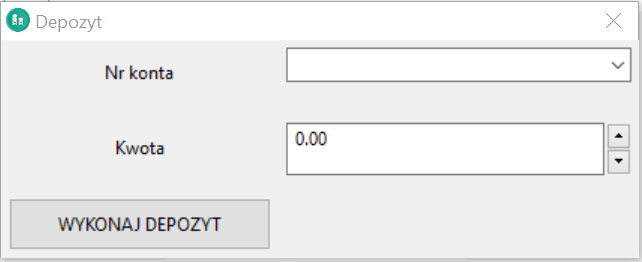
\includegraphics[width=0.8\textwidth]{depozyt.png}
	\caption{Depozyt}
	\label{depozyt}
\end{figure}
\newpage
\subsection{Kod źródłowy}
Funkcja sprawdza poprawność wybranego numeru konta, aktualizuje saldo konta o podaną kwotę depozytu, a następnie informuje użytkownika o wyniku operacji.
\begin{lstlisting}
void wxDepozyt::deposit(wxCommandEvent& event)
	{ if (ComboBox1->wxItemContainerImmutable::IsEmpty()) {
			wxMessageBox("Pole jest puste.", "Blad", wxICON_ERROR);
			return;
		} else if (!ComboBox1->GetValue().IsNumber()) {
			wxMessageBox("Pole numer moze zawierac tylko liczby.", "Blad", wxICON_ERROR);
			return; }
		int option = 1;
		int number = stoi(w2s(ComboBox1->GetValue()));
		double amount = SpinCtrlDouble1->GetValue();
		
		fstream file(filePath);
		ofstream tempFile(tempFilePath);
		string line;
		bool found = false;
		while (getline(file, line)) {
			istringstream iss(line);
			int currentAccountNumber;
			string name, surname;
			double balance;
			iss >> currentAccountNumber >> name >> surname >> balance;
			if (currentAccountNumber == number) {
				if (option == 1) {
					balance += amount;
					found = true;
				} else {
					if (amount <= balance) {
						balance -= amount;
						found = true;
					} else {
						break;
					}
				}
			}
			tempFile << currentAccountNumber << '\t' << name << '\t' << surname << '\t' << balance << '\n';
		}
		file.close();
		tempFile.close();
		if (found && wxRenameFile(tempFilePath, filePath, true)) {
			wxMessageBox(_("Saldo zostalo pomyslnie zaktualizowane."), wxMessageBoxCaptionStr, wxICON_INFORMATION);
			globalComboBoxItems.erase(std::find(globalComboBoxItems.begin(), globalComboBoxItems.end(), wxString::Format("%d", number)));
			globalComboBoxItems.insert(globalComboBoxItems.begin(), wxString::Format("%d", number));
			Close(true);
		} else {
			wxMessageBox(_("Nie znaleziono konta lub wystapil blad podczas aktualizacji salda."), "Error", wxICON_ERROR);
			wxRemoveFile(tempFilePath);
		}
	}
\end{lstlisting}

	\section{Wycofanie środków z konta}
	Wycofanie środków z konta (odebraniu określonej kwoty) jest możliwe do zrobienia postępując wobec podanych niżej czynności:
	\begin{enumerate}
		\item Otworzyć aplikację bankowości
		\item Kliknąć przycisk ‘\textbf{WYCOFAJ ŚRODKI}’
		\item W polu „Nr konta” wpisać numer konta użytkownika
		\item W polu „Kwota” wpisać kwotę, o ile powinien zmniejszyć się stan konta użytkownika
		\item Kliknąć przycisk ‘\textbf{WYCOFAJ ŚRODKI}’ po wprowadzeniu i weryfikacji danych 
	\end{enumerate}
\begin{figure}[h]
	\centering
	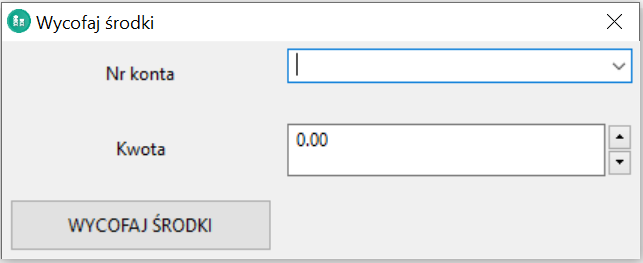
\includegraphics[width=0.8\textwidth]{wycofaj.png}
	\caption{Wycofanie środków}
	\label{wycofaj}
\end{figure}
	\subsection{Kod źródłowy}
	Funkcja jest odpowiedzialna za wypłatę środków z konta w aplikacji bankowej. Sprawdza poprawność numeru konta i kwoty wypłaty, aktualizuje saldo konta o odpowiednią kwotę, a następnie informuje użytkownika o wyniku operacji.
	\begin{lstlisting}
void wxWycofaj::withdraw(wxCommandEvent& event)
		{ if (ComboBox1->wxItemContainerImmutable::IsEmpty()) {wxMessageBox("Pole jest puste.", "Blad", wxICON_ERROR);
				return;
			} else if (!ComboBox1->GetValue().IsNumber()) {wxMessageBox("Pole numer moze zawierac tylko liczby.", "Blad", wxICON_ERROR);
				return; }
			int option = 0;
			int number = stoi(w2s(ComboBox1->GetValue()));
			double amount = SpinCtrlDouble1->GetValue();
			fstream file(filePath);
			ofstream tempFile(tempFilePath);
			string line;
			bool found = false;
			while (getline(file, line)) {
				istringstream iss(line);
				int currentAccountNumber;
				string name, surname;
				double balance;
				iss >> currentAccountNumber >> name >> surname >> balance;
				if (currentAccountNumber == number) {
					if (option == 1) {
						balance += amount;
						found = true;
					} else {
						if (amount <= balance) {
							balance -= amount;
							found = true;
						} else {
							break;}}}
				tempFile << currentAccountNumber << '\t' << name << '\t' << surname << '\t' << balance << '\n';}
			file.close();
			tempFile.close();
			if (found && wxRenameFile(tempFilePath, filePath, true)) {
				wxMessageBox(_("Saldo zostalo pomyslnie zaktualizowane."), wxMessageBoxCaptionStr, wxICON_INFORMATION);
				globalComboBoxItems.erase(std::find(globalComboBoxItems.begin(), globalComboBoxItems.end(), wxString::Format("%d", number)));
				globalComboBoxItems.insert(globalComboBoxItems.begin(), wxString::Format("%d", number));
				Close(true);
			} else {
				wxMessageBox(_("Nie znaleziono konta lub kwota jest wieksza od salda."), "Blad", wxICON_ERROR);
				wxRemoveFile(tempFilePath);}}
	\end{lstlisting}

	\section{Sprawdzenie salda konta}
	Chcąc sprawdzić saldo konkretnego konta użytkownika należy:
	\begin{enumerate}
		\item Otworzyć aplikację bankowości
		\item Kliknąć przycisk ‘\textbf{SALDO KONTA}’
		\item W polu „Nr konta” wpisać numer konta użytkownika
		\item Kliknąć przycisk ‘\textbf{POKAŻ STAN KONTA}’ po wprowadzeniu i weryfikacji danych
	\end{enumerate}

\begin{figure}[h]
	\centering
	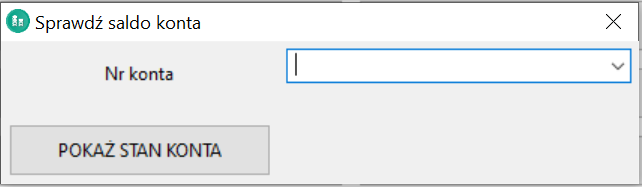
\includegraphics[width=0.8\textwidth]{saldo.png}
	\caption{Sprawdzenie salda konta}
	\label{saldo}
\end{figure}
\newpage
\subsection{Kod źródłowy}

Funkcja sprawdza saldo wybranego konta w aplikacji bankowej. Jeśli numer konta jest poprawny i istnieje w pliku danych, wyświetla aktualne saldo. W przeciwnym razie informuje użytkownika o braku konta lub nieprawidłowym numerze.
	\begin{lstlisting}
void wxSaldo::OnButton1Click(wxCommandEvent& event)
		{if (ComboBox1->wxItemContainerImmutable::IsEmpty()) {wxMessageBox("Pole jest puste.", "Blad", wxICON_ERROR);
			return;
			} else if (!ComboBox1->GetValue().IsNumber()) { wxMessageBox("Pole numer moze zawierac tylko liczby.", "Blad", wxICON_ERROR);
			return; }
		int num = stoi(w2s(ComboBox1->GetValue()));
		ifstream file(filePath);
		string line;
		bool found = false;
		while (getline(file, line)) {istringstream iss(line);
			int currentAccountNumber;
			string name, surname;
			double balance;
		iss >> currentAccountNumber >> name >> surname >> balance;
			if (currentAccountNumber == num) {
		wxString balanceString = wxString::Format(_("%.1f"), balance);
			wxMessageBox(_("Saldo: ") + balanceString, wxMessageBoxCaptionStr, wxICON_INFORMATION);
			found = true;
			globalComboBoxItems.erase(std::find(globalComboBoxItems.begin(), globalComboBoxItems.end(), wxString::Format("%d", num)));
			globalComboBoxItems.insert(globalComboBoxItems.begin(), wxString::Format("%d", num));
			Close(true);
			break;}}
			file.close();
			if (!found) {
				wxMessageBox(_("Konto nie znalezione."), "Error", wxICON_ERROR);}}
	\end{lstlisting}
\newpage
	\section{Zlecenie przelewu między kontami}
	Przelew jest najważniejszą operacją związaną z bankowością. Aby zlecić przelew między kontami potrzeba:
\begin{enumerate}
	\item Otworzyć aplikację bankowości
	\item Kliknąć przycisk ‘\textbf{ZLEĆ PRZELEW}’
	\item W polu „Nr konta nadawcy” wpisać numer konta użytkownika nadającego przelew
	\item W polu „Nr konta odbiorcy” wpisać numer konta użytkownika odbierającego przelew
	\item W polu „Kwota” wpisać kwotę przelewu
	\item Kliknąć przycisk ‘\textbf{WYKONAJ PRZELEW}’ po wprowadzeniu i weryfikacji danych
\end{enumerate}

\begin{figure}[h]
	\centering
	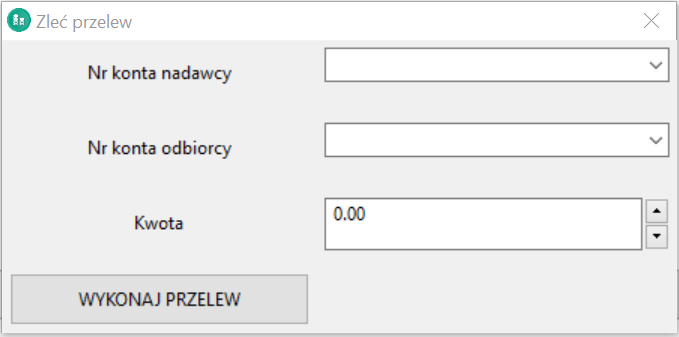
\includegraphics[width=0.8\textwidth]{przelew.png}
	\caption{Zlecenie przelewu}
	\label{Przelew}
\end{figure}

\subsection{Kod źródłowy}
Funkcja zajmuje się operacją przekazywania środków między kontami w aplikacji bankowej. Sprawdza poprawność danych wejściowych, w tym numerów kont oraz dostępnych środków na koncie źródłowym. Następnie aktualizuje saldo kont zaangażowanych w transakcję i informuje użytkownika o wyniku operacji.
\begin{lstlisting}
void wxPrzelew::transaction(wxCommandEvent& event)
	{if (ComboBox1->wxItemContainerImmutable::IsEmpty() || ComboBox2->wxItemContainerImmutable::IsEmpty()) {wxMessageBox("Pole jest puste.", "Blad", wxICON_ERROR);
			return;
		} else if (!ComboBox1->GetValue().IsNumber() || !ComboBox2->GetValue().IsNumber()) {wxMessageBox("Pole numer moze zawierac tylko liczby.", "Blad", wxICON_ERROR);
			return;}
		int num = stoi(w2s(ComboBox1->GetValue()));
		int recipient = stoi(w2s(ComboBox2->GetValue()));
		double amount = SpinCtrlDouble1->GetValue();
		fstream file(filePath);
		ofstream tempFile(tempFilePath);
		string line;
		bool sourceAccountFound = false;
		bool destinationAccountFound = false;
		double sourceBalance;
		while (getline(file, line)) {
			istringstream iss(line);
			int currentAccountNumber;
			string name, surname;
			double balance;
			iss >> currentAccountNumber >> name >> surname >> balance;
			if (currentAccountNumber == num) {
				sourceAccountFound = true;
				sourceBalance = balance;
				if (amount <= sourceBalance) {
					balance -= amount;
					tempFile << currentAccountNumber << '\t' << name << '\t' << surname << '\t' << balance << '\n';
				} else {
					wxMessageBox(_("Konto zrodlowe nie ma wystarczajacego salda dla transakcji."), "Blad", wxICON_ERROR);
					tempFile << line << '\n';
					file.close();
					tempFile.close();
					wxRemoveFile(tempFilePath);
					return;}
			} else if (currentAccountNumber == recipient) {
				destinationAccountFound = true;
				balance += amount;
				tempFile << currentAccountNumber << '\t' << name << '\t' << surname << '\t' << balance << '\n';
			} else {
				tempFile << currentAccountNumber << '\t' << name << '\t' << surname << '\t' << balance << '\n';	}}
		file.close();
		tempFile.close();
		if (sourceAccountFound && destinationAccountFound && wxRenameFile(tempFilePath, filePath, true)) {wxMessageBox(_("Transakcja zakonczona pomyslnie."), wxMessageBoxCaptionStr, wxICON_INFORMATION);
			globalComboBoxItems.erase(std::find(globalComboBoxItems.begin(), globalComboBoxItems.end(), wxString::Format("%d", num)));
			globalComboBoxItems.insert(globalComboBoxItems.begin(), wxString::Format("%d", num));
			globalComboBoxItems.erase(std::find(globalComboBoxItems.begin(), globalComboBoxItems.end(), wxString::Format("%d", recipient)));
			globalComboBoxItems.insert(globalComboBoxItems.begin(), wxString::Format("%d", recipient));
			Close(true);
		} else {
			wxMessageBox(_("Blad podczas wykonywania transakcji."), "Blad", wxICON_ERROR);
			wxRemoveFile(tempFilePath);}}
\end{lstlisting}
	\section{Wyświetlenie listy kont}
	Wyświetlenie listy wszystkich kont jest osiągalne poprzez następujące czynności:
	\begin{enumerate}
		\item Otworzyć aplikację bankowości
		\item Kliknąć przycisk ‘\textbf{LISTA KONT}’
	\end{enumerate}

\begin{figure}[h]
	\centering
	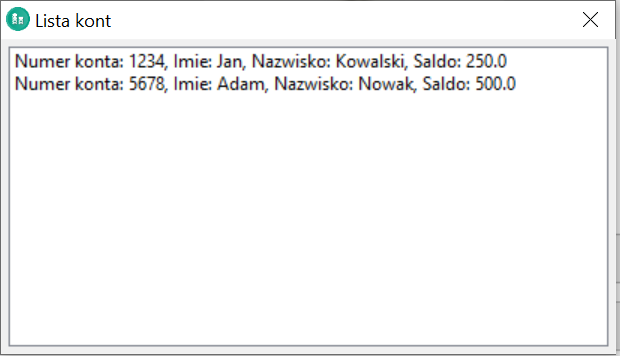
\includegraphics[width=0.8\textwidth]{lista.png}
	\caption{Lista z przykładowymi kontami}
	\label{lista}
\end{figure}
\subsection{Kod źródłowy}
Odpowiada za tworzenie listy kont w aplikacji bankowej. Najpierw inicjuje okno dialogowe o tytule "Lista kont", w którym znajduje się przewijalne okno (ScrolledWindow1) oraz lista (ListBox1). Następnie, wczytuje dane z pliku "db.txt" zawierające informacje o numerze konta, imieniu, nazwisku i saldzie. Te informacje są dodawane do listy kont. Jeśli lista jest pusta, użytkownik otrzymuje komunikat informujący o braku danych.
\begin{lstlisting}
wxLista::wxLista(wxWindow* parent,wxWindowID id,const wxPoint& pos,const wxSize& size)
	{wxString filename = "db.txt";
		ifstream file(filename.ToStdString());
		ListBox1->Clear();
		string line;
		wxArrayString entries;
		while (getline(file, line)) {istringstream iss(line);
			int number;
			string name, surname;
			double balance;
		if (iss >> number >> name >> surname >> balance) {wxString entry = wxString::Format("Numer konta: %d, Imie: %s, Nazwisko: %s, Saldo: %.1f",
			number, name, surname, balance);
			entries.Add(entry);}}
		file.close();
		if (!entries.IsEmpty()) {
			ListBox1->InsertItems(entries, 0);
		} else {
		ListBox1->Append("Brak wpisow w bazie danych."); }}
\end{lstlisting}
	\section{Modyfikacja danych}
	W celu zaktualizowania danych takich jak imię, nazwisko lub saldo konta, należy:
	\begin{enumerate}
		\item Otworzyć aplikację bankowości
		\item Kliknąć przycisk ‘\textbf{MODYFIKUJ INFORMACJE}’
		\item W polu „Nr konta” wpisać numer konta użytkownika, którego dane będą zmieniane
		\item W polu „Imię” wpisać niezmienione lub zaktualizowane imię użytkownika
		\item W polu „Nazwisko” wpisać niezmienione lub zaktualizowane nazwisko użytkownika
		\item W polu „Saldo konta” wpisać niezmienione lub zaktualizowane saldo konta użytkownika
		\item Kliknąć przycisk ‘\textbf{MODYFIKUJ}’ po wprowadzeniu i weryfikacji danych
	\end{enumerate}
	\begin{figure}[h]
		\centering
		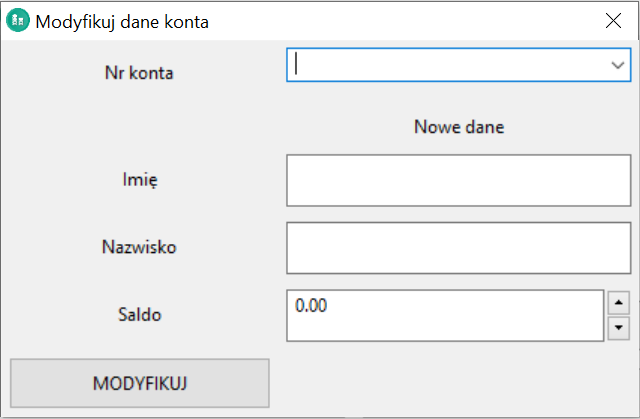
\includegraphics[width=0.8\textwidth]{modyfikuj.png}
		\caption{Modyfikacja danych konta}
		\label{modyfikuj}
	\end{figure}
	\subsection{Kod źródłowy}
	Funkcja modyfikuje dane konta w interfejsie aplikacji bankowej. Sprawdza poprawność danych wejściowych, a następnie aktualizuje plik. Po udanej operacji informuje użytkownika o pomyślnej modyfikacji konta, a w przypadku błędu wyświetla stosowny komunikat.
	\begin{lstlisting}
void wxModyfikuj::modify_account(wxCommandEvent& event)
		{if (ComboBox1->wxItemContainerImmutable::IsEmpty() || TextCtrl2->IsEmpty() || TextCtrl3->IsEmpty()) {
				wxMessageBox("Pole jest puste.", "Blad", wxICON_ERROR);
				return;
			} else if (!ComboBox1->GetValue().IsNumber()) {
				wxMessageBox("Pole numer moze zawierac tylko liczby.", "Blad", wxICON_ERROR);
				return;	}
			int num = stoi(w2s(ComboBox1->GetValue()));
			int new_balance = SpinCtrlDouble1->GetValue();
			string new_name = w2s(TextCtrl2->GetValue());
			string new_surname = w2s(TextCtrl3->GetValue());
			fstream file(filePath);
			ofstream tempFile(tempFilePath);
			string line;
			bool found = false;
			while (getline(file, line)) {
				istringstream iss(line);
				int currentAccountNumber;
				string name, surname;
				double balance;
				iss >> currentAccountNumber >> name >> surname >> balance;
				if (currentAccountNumber == num) {
					found = true;
					tempFile << currentAccountNumber << '\t' << new_name << '\t' << new_surname << '\t' << new_balance << '\n';
				} else {
					tempFile << currentAccountNumber << '\t' << name << '\t' << surname << '\t' << balance << '\n';}}
			file.close();
			tempFile.close();
			if (found && wxRenameFile(tempFilePath, filePath, true)) {
				wxMessageBox(_("Konto zostalo pomyslnie zmodyfikowane."), wxMessageBoxCaptionStr, wxICON_INFORMATION);
				globalComboBoxItems.erase(std::find(globalComboBoxItems.begin(), globalComboBoxItems.end(), wxString::Format("%d", num)));
				globalComboBoxItems.insert(globalComboBoxItems.begin(), wxString::Format("%d", num));
				Close(true);
			} else {
				wxMessageBox(_("Nie znaleziono konta lub wystapil blad podczas modyfikowania konta."), "Error", wxICON_ERROR);
				wxRemoveFile(tempFilePath);}}
	\end{lstlisting}
	\section{Usuwanie konta bankowego}
	Aby usunąć konto bankowe użytkownika trzeba postępować według poniższych kroków:	
	\begin{enumerate}
	\item Otworzyć aplikację bankowości
	\item Kliknąć przycisk ‘\textbf{USUŃ KONTO}’
	\item W polu „Nr konta” wpisać numer konta użytkownika, którego konto zostanie usunięte
	\item Kliknąć przycisk ‘\textbf{POTWIERDŹ}’ po wprowadzeniu i weryfikacji danych
\end{enumerate}
\begin{figure}[h]
	\centering
	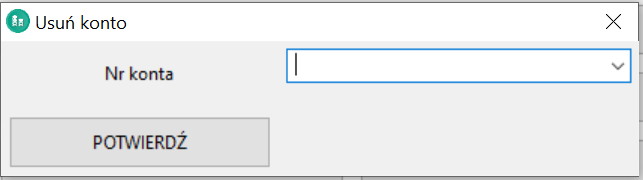
\includegraphics[width=0.8\textwidth]{usun.png}
	\caption{Usuwanie konta}
	\label{usun}
\end{figure}
\newpage
\subsection{Kod źródłowy}
Funkcja usuwa konto z aplikacji bankowej. Sprawdza poprawność danych wejściowych, a następnie aktualizuje plik. Po udanej operacji informuje użytkownika o pomyślnym usunięciu konta, a w przypadku błędu wyświetla stosowny komunikat.
\begin{lstlisting}
void wxUsun::delete_account(wxCommandEvent& event)
	{if (ComboBox1->wxItemContainerImmutable::IsEmpty()){ wxMessageBox("Pole jest puste.", "Blad", wxICON_ERROR);
			return;
		} else if (!ComboBox1->GetValue().IsNumber()) {
			wxMessageBox("Pole numer moze zawierac tylko liczby.", "Blad", wxICON_ERROR);
			return; }
		int num = stoi(w2s(ComboBox1->GetValue()));
		fstream file(filePath);
		ofstream tempFile(tempFilePath);
		string line;
		bool found = false;
		while (getline(file, line)) {
			istringstream iss(line);
			int currentAccountNumber;
			string name, surname;
			double balance;
			iss >> currentAccountNumber >> name >> surname >> balance;
			if (currentAccountNumber == num) {
				found = true;
			} else {
				tempFile << currentAccountNumber << '\t' << name << '\t' << surname << '\t' << balance << '\n';	}}
		file.close();
		tempFile.close();
		if (found && wxRenameFile(tempFilePath, filePath, true)) {
			wxMessageBox(_("Konto usuniete pomyslnie."), wxMessageBoxCaptionStr, wxICON_INFORMATION);
			globalComboBoxItems.erase(std::find(globalComboBoxItems.begin(), globalComboBoxItems.end(), wxString::Format("%d", num)));
			Close(true);
		} else {
			wxMessageBox(_("Nie znaleziono konta lub wystapil blad podczas usuwania konta."), "Blad", wxICON_ERROR);
			wxRemoveFile(tempFilePath);	}}
\end{lstlisting}
	\section{Podział pracy}
	\begin{itemize}
		\item 	GUI - Magdalena Denicka 100 \%
		\item Plan projektu - Magdalena Denicka 50\%, Andrii Zapukhlyi 50\%
		\item Funkcjonalność i praca z bazą danych - Andrii Zapukhlyi 100\%
		\item Dokumentacja - Magdalena Denicka 100\%
	\end{itemize}

	\listoffigures
	
\end{document}
